%%%%%%%%%%%%%%%%%%%%%%%%%%%%%%%%%%%%%%%%%%%%%%%%%%%%%%%%%%%%%%%%%%%%%%%%%%%%%%%%
\section{Cryptographic Hash Functions}
\label{sec:hashfunctions}

\begin{wrapfigure}{r}{2in}
  \centering
    \begin{tikzpicture}[scale=0.4]
        \node[draw,trapezium,trapezium left angle=70,trapezium right angle=70,minimum height=1.0cm,thick,shift={(1.15,0)},rotate=-90] (hfxn)
        {\begin{sideways}\Large $\hash$ \end{sideways}};
        \draw[->,thick] (0,0) node[left] {$M$} -- (hfxn);
        \draw[->,thick] (hfxn) -- ++(3,0) node[right] {$H(M)$};
    \end{tikzpicture}
    \caption{An abstract hash function, where $M$ is the message and $H(M)$ the corresponding hash (or ``digest'')}
\label{fig:hash-function}
\end{wrapfigure}

A \emph{cryptographic hash function (CHF)} is a map $H\Colon\msgspace\rightarrow\bits^n$, i.e. deterministic function, for
some set $\msgspace$ and number $n > 0$. 
CHFs are a highly useful building blocks for secure applications, because the allow to derive a concise integer representation, that is hard to forge, from an arbitrary large input message.
Typical values of $n$ these days are 256, 512, or 1024, and most hash functions support an essentially unlimited message space $\msgspace$, such as all strings of length up to $2^{64}-1$.

CHFs enable us to prove the integrity or existence of a binary blob without having to transfer the entire data, which allows to increase efficiency in many use cases. They further are hard to inverse, i.e. it is non-trivial to derive the input value (or \emph{message}) from the hash value (or \emph{digest}).
Applications of CHFs include, but are not limited to, file comparison, digital signatures, message authenticated codes, key derivation, password hashing.

\subsection{Collision Resistance}
Collision resistance is a core property of hash functions.
This property guarantees that it is very hard for an adversary to find two messages that correspond to the same hash, which ensures that the same cryptographic signature cannot be reused by an attacker for a different message.

\begin{wrapfigure}{r}{2in}
\fpage{.3}{
    \underline{$\advA_{Cr}$}\\[1pt]
For i = 1 to q do: \\
\myInd $X_i \getsr {\{0, 1\}}^m$\\
\myInd $h_i \leftarrow H(X_i)$\\
If $\exists i,j$ s.t. $X_i \neq X_j \land h_i \neq h_j$ then\\
\myInd Return $(X_i, X_j)$\\
Return \false
}
\end{wrapfigure}


On a high level, the \emph{pigeonhole principle} states that functions that map from a large space there exists an efficient adversary that is able to find a collision.
However, Rogaway showed that these are non-trivial to find for a human adversary~\cite{rogaway2006formalizing}.
Thus, the birthday attack is most efficient known attack against cryptographic hash functions and will be described in the following.

\begin{theorem*}
For a regular hash function, probability that an attacker $A_{Cr}$ finds a collision is $\ge 0.3 \frac{q(q-1)}{2^n}$, where $q$ is the number of messages queried by $A_{Cr}$.
\end{theorem*}

\begin{proof}
    $A_{Cr}$ picks $q$ messages independently at random. We can then derive the probability that a collision is found after $A_{Cr}$ ran as the following. Here ${Coll}_i$ represents the probability that a chosen value $Y_i$ is equal to a previous value $Y_j$.

\begin{align*}
    Pr[Coll] = Pr[{Coll}_1 \lor {Coll}_2 \lor \dots \lor {Coll}_q] \\
             \geq Pr[{Coll}_1] + Pr[{Coll}_2] + \dots + Pr[{Coll}_q] \\
             = \frac{0}{2^n} + \frac{1}{2^n} + \dots + \frac{q}{2^n} \\
             = \frac{q(q-1)}{2^n}
\end{align*}

For a regular hash function this bound is even tighter.
We define regular in this context as the property that each point in the range of the function maps to the same number of input points.
In other words, each point in the range has the same number of pre-images (see Section \ref{sec:hashfunctions2} for a discussion on pre-images and pre-image resistance).
In this case the bound is equal to the regular birthday probability~\scribenote{Do we need a proof for that? I was not able to find one}.

$$
    Pr[Coll] \geq 0.3 \frac{q(q-1)}{2^n}
$$
\end{proof}

\subsection{Building a Cryptographic Hash Function}
\begin{wrapfigure}{r}{2in}
    \centering
\fpage{.25}{
    \underline{$\advA(K)$}\\[1pt]
$M \leftarrow E_k(0^n) \xor E_k(1^n) $ \\
Return $(0^n 0^n, 1^n || M)$
}
    \caption{An efficient attacker for a CBC-MAC-based hash function.}
    \label{fig:cbc-hash-attack}
\end{wrapfigure}

Now that we discussed some of the guarantees of CHFs, we will investigate how to build such a primitive.
Ideally, we would like to leverage building blocks that were introduced in previous parts of these notes.
CBC-MAC, like CHFs, takes a variable size input and converts it into a fixed size value.
In the following we discuss why CBC-MAC is \emph{not} a good hash function.


To show that CBC-MAC is unfit to be used as CHF, we sketch an efficient attack to find a hash collision.
    Our attacker $A$ (outlined in Figure \ref{fig:cbc-hash-attack}) leverages the fact that ever step of CBC-MAC uses the same encryption key, which is must be public in order to use CBC-MAC as a hash function.
$A$ then aims to compute to input values that are each two blocks wide and map to the same hash.
Here, CBC-MAC will invoke the underlying encryption function twice.
Because the encryption key is identical in both cases, all we have to ensure is that the value passed to the second encryption pass is identical as well in both cases.

To generate an identical input value, we need to cancel out the output of the first encryption pass.
$A$ achieves this by first computing the desired output with the expected output. 
Setting the XOR of the two as the second part of the message will cancel out the expected, and undesired, output of the previous function.
Here, the input for the second encryption pass is $E_k(0^n) \xor E_k(1^n) \xor E_k(1^n) = E_k(0^n)$. $\qed$

\begin{wrapfigure}{r}{2.9in}
\begin{tikzpicture}[scale=0.4]
	\begin{scope}[]
		\node [draw,trapezium,trapezium left angle=50,trapezium right angle=90,minimum height=0.75cm,thick,shift={(1.15,0.3)},rotate=-90]
		{\begin{sideways}\Large$f$\end{sideways}};
		\draw[->,thick] ++(0.5,+4) node[above] {$\msg_1$} -- ++(0,-1.5) -- ++(1.4,0);
		\draw[->,thick] ++(0,0.5) node[left] {$\IV$} -- ++(1.9,0);
	\end{scope}

	\begin{scope}[shift={(3.8,0)}]
		\node [draw,trapezium,trapezium left angle=50,trapezium right angle=90,minimum height=0.75cm,thick,shift={(1.35,0.3)},rotate=-90] (centerbox)
		{\begin{sideways}\Large$f$\end{sideways}};
		\draw[->,thick] ++(0.9,+4) node[above] {$\msg_2$} -- ++(0,-1.5) -- ++(1.4,0);
		\draw[->,thick] ++(0,0.5) -- ++(2.4,0);
	\end{scope}

	\begin{scope}[shift={(8.2,0)}]
		\node [draw,trapezium,trapezium left angle=50,trapezium right angle=90,minimum height=0.75cm,thick,shift={(1.35,0.3)},rotate=-90]
		{\begin{sideways}\Large$f$\end{sideways}};
		\draw[->,thick] ++(0.9,+4) node[above] {$\qquad\msg_3 \concat 10^r \concat \bm{\langle} \left| \msg \right| \bm{\rangle}$} -- ++(0,-1.5) -- ++(1.4,0);
		\draw[->,thick] ++(0,0.5) -- ++(2.4,0);
        \draw[->,thick] ++(4.4,0.5) -- ++(2,0) node[right] {$H(M)$};
	\end{scope}
\end{tikzpicture}
\caption{A sketch of the Merkle-Damgard Construction}
\label{fig:md-construction}
\end{wrapfigure}

\paragraph{}
We now introduce the \emph{Merkle-Damgard Construction}, which uses a similar scheme except that it changes the encryption key in every step.
The MD-construction changes the key on every step by inputting the respective part of the message as the encryption key, while the input and output of the encryption function are used to maintain state of the hashing process.
Figure \ref{fig:md-construction} outlines this scheme in more detail.

While this design seems promising, it is still prone to prefix attacks, similar to the one outlined before, when using a plain block cipher as compression function.
This means, in order to make the MD-construction safe, we need to find a better compression function.
Compression functions are a one-way function like hash functions, but, unlike hash functions, they take a constant-size block as well as a constant-size state as input, both of which must be hard to derive from the output alone.

The \emph{Davies-Meyers compression function}~\cite{winternitz1984secure,black2002black} is constructed by modifying wrapping a block cypher.
It adds a XOR operation of the encryption output with the input state before the encryption.
This makes it hard to regenerate $E_K$'s input even when knowing $K$ if $E_K$ is an \emph{ideal block cipher}.
We define ideal block ciphers, as ciphers where each key generates an new random permutation independent of those generated by other keys.
In other words, it is very unlikely that an ideal block cipher maps one input to the same output under different keys.

\begin{wrapfigure}{r}{2.9in}
\centering
    \begin{tikzpicture}[scale=0.4]
        \node (M) {M};
        \node [right=0.5cm of M] (M2) {};
        \node [below=1cm of M2.center] (M3) {};
        \node [right=0.5cm of M2, draw,rectangle, minimum width=1.5cm, minimum height=0.75cm,thick] (E) {$E_K$};
        \node [right=0.5cm of E, draw, circle, inner sep=-1, outer sep=0] (xor) {$\xor$};
        \node [below=1cm of xor.center] (xor2) {};
        \node [right=0.5cm of xor] (Y) {};
        \draw[thick] (M) -- (M2.center);
        \draw[->, thick] (M2.center) -- (E);
        \draw[thick] (M2.center) -- (M3.center);
        \draw[thick] (M3.center) -- (xor2.center);
        \draw[thick] (E) -- (xor);
        \draw[thick] (xor2.center) -- (xor);
        \draw[->, thick] (xor) -- (Y);
    \end{tikzpicture}
\caption{The Davies-Meyers compression function}
\end{wrapfigure}

\begin{wrapfigure}{l}{2.6in}
\fpage{.25}{
\underline{$\CR^\advA_{H}$}\\[1pt]
$(M,M') \getsr \advA$\\
If $M = M'$ then Ret $\false$\\
Ret $H(M) = H(M')$
}

\bnm
\AdvCR{H}{\advA} = \Prob{\CR^\advA_H\Rightarrow\true}
\enm

\fpage{.25}{
\underline{$\CR^\advA_{H,\ic}$}\\[1pt]
$(E, D) \getsr \blockciphers(k,n)$\\
$(M,M') \getsr \advA^{\ic,\icInv}$\\
If $M = M'$ then Ret $\false$\\
Ret $H^\ic(M) = H^\ic(M')$\medskip

\underline{$\ic(K,X)$}\\
Ret $\cipherE(K,X)$\medskip

\underline{$\icInv(K,Y)$}\\
Ret $\cipherD(K,Y)$
}
\end{wrapfigure}

\begin{theorem*}
Let $f$ be the Davies-Meyer compression function built from a block cipher
$\cipherE\Colon\bits^k\times\bits^n\rightarrow\bits^n$ modeled as an ideal
cipher and let $D$ be the associated decryption function.
For any adversary $\advA$ making at most~$q$ queries it holds that
\bnm
  \AdvCR{f}{\advA} \le \frac{(q+1)(q+2)}{2^n} \;.
\enm
\end{theorem*}

\paragraph{Proof}
Assume $\advA$ that outputs $(Y,M)$ and $(Y',M')$ has already queried $\cipherE$ or $\cipherD$ for associated points.
This can be argued easily by reducing $\advA$ to making at most $q' = q+2$ queries.
Then each query defines a triple $(K_i,X_i,Y_i)$ where either $Y_i = \cipherE(K_i,X_i)$ was queried or $X_i =
\cipherD(K_i,Y_i)$ was queried. For a collision to occur it must be that there
exist indices $i,j$ such that $X_i \oplus Y_i = X_j \oplus Y_j$, to arrange that
$X_i \oplus \cipherE(K_i,X_i) = X_j \oplus \cipherE(K_j,X_j)$. Let $C_j$ be the
event that such a collision occurs upon a query the $j\thh$ query. Then we have
that $X_i,Y_i$ are at this point fixed values while exactly one of $X_j$ or
$Y_j$ is a fixed value, with the other being a uniformly chosen point subject
only to permutivity. Then we have that 
\begin{align*}
\Prob{\CR_{f,\cipherE}^\advA\Rightarrow\true} 
    &\le \sum_{j=1}^{q'} \Prob{C_j}  &  \\
    &\le \sum_{j=1}^{q'} \frac{j-1}{2^n-j+1} &\\
    &\le \sum_{j=1}^{q'} \frac{j-1}{2^n-q'} &\\
    &= \frac{q'(q'-1)}{2(2^n-q')} & \\
    &\le \frac{(q+2)(q+1)}{2^n} &( \text{assuming }q' \leq 2^{n-1} ) \\
\end{align*}

Which let's us conclude that the theorem holds. $\qed$

\newpage %manual formatting, remove if not needed anymore

\subsubsection{SHA-1}
\begin{wrapfigure}{r}{5cm}
    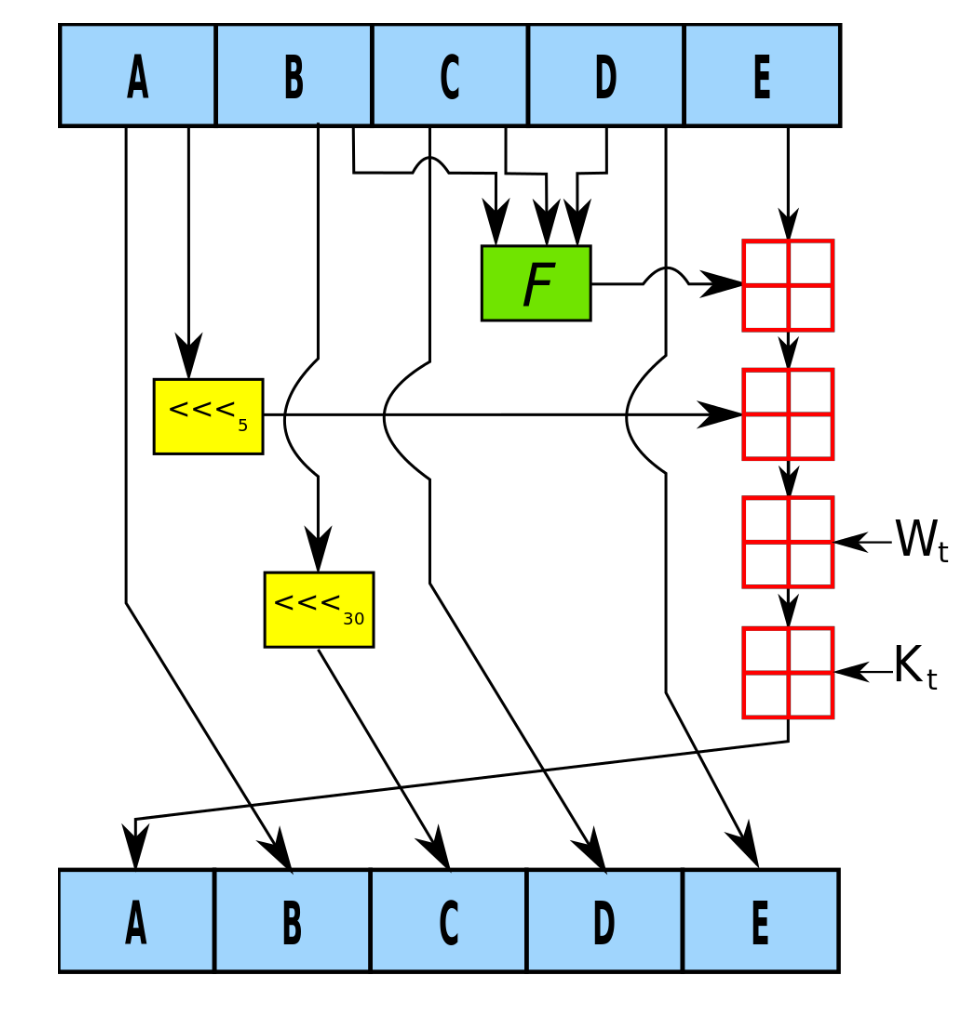
\includegraphics[width=5cm]{hash/sha1}
    \caption{One round of SHA-1}
    \label{fig:sha1}
\end{wrapfigure}

SHA-1 (for \emph{secure hash standard}) is a widely used cryptographic hash function that relies on the principles introduced previously.
It performs 80 rounds of a variant of the Davies-Meyers construction.

Figure \ref{fig:sha1} outlines the SHA-1 scheme. Each run of SHA-1 processes blocks of 512 bits, which are split into 80 32-bit values ($W_t$).
The scheme maintains a 160-bit chaining variable ($A$ to $F$).
Note, that instead of an existing block cipher (e.g. AES) a custom block cipher is used, that takes the chaining variable, $W_t$, as well as a round constant ($K_t$) as input.
To understand why this custom scheme is advantageous, let use recall that crytographic hash functions aim for small changes in the input to lead to large changes in the output.
For the Davies-Meyers construction this means that the block cipher must be resilient to so-called related-key attacks, however it has been shown by Biryukov et al.~\cite{biryukov2009related} that AES is not. 

\subsection{Attacks on MD5 and SHA-1}
\begin{table}[htb]
\centering
    \begin{tabular}{|c|c|c|}
        \hline
        2004 & MD5 is broken & Wang et al.~\cite{wang2005break} \\
        2005 & Theoretical attacks on SHA-1 & Wang et al.~\cite{wang2005finding} \\
        2017 & First practical attack on SHA-1 & CWI and Google~\cite{stevens2017first} \\
        \hline
    \end{tabular} \\
    \scribenote{should we add more stuff here, not mentioned in the lecture?}
    \caption{Timeline of attacks on SHA-1 and MD5}
\end{table}

SHA-1 and it's predecessors MD5 are vulnerable to certain attacks.
While MD5 has been shown to be vulnerable in a real-life settings as early as 2004, it took until 2017 to show a practical attack on SHA-1.
However, because theoretical attacks to SHA-1 have been shown as early as 2005, industry has already deprected SHA-1 and moved on to new standards.
In particular, SHA-2 and SHA-3 have been introduced. The latter will be described in the next section.




\subsection*{Exercises}
\begin{figure}[htb]
\begin{tikzpicture}[scale=0.4]
    \node (M) {M};
    \node [right=0.5cm of M, draw, circle, inner sep=-1, outer sep=0] (xor) {$\xor$};
    \node [below=1cm of xor.center] (xor2) {};
    \node [right=0.5cm of xor, draw,rectangle, minimum width=1.5cm, minimum height=0.75cm,thick] (E) {$E_K$};
    \node [right=0.5cm of E] (M2) {};
    \node [below=1cm of M2.center] (M3) {};
    \node [right=0.5cm of M2.center] (Y) {};
    \draw[thick, ->] (M) -- (xor);
    \draw[thick] (xor) -- (xor2.center);
    \draw[thick] (xor2.center) -- (M3.center);
    \draw[thick] (M3.center) -- (M2.center);
    \draw[thick] (E) -- (M2.center);
    \draw[->, thick] (xor) -- (E);
    \draw[->, thick] (M2.center) -- (Y);
\end{tikzpicture}
    \caption{An alternative to the Davies-Meyers construction?}
    \label{fig:dm-alt-construction}
\end{figure}

\begin{enumerate}[label=\textbf{Exercise \thesection.\arabic*}, wide=0pt]
    \item Consider Figure \ref{fig:dm-alt-construction} as an alternative to the Davies-Meyers construction. Can it be used to build a CHF? If not, why?
    \item Consider a hash function \texttt{POWSHA(M, k)} that takes a message and a public constant $k$. \texttt{POWSHA} applies \texttt{SHA-1} to $M$ and then recursively calls \texttt{SHA-1} on the output $k-1$ times. How much safer is this construction compared to \texttt{SHA-1}?
\end{enumerate}

\scribenote{These are too easy but I cannot come up withe something harder for this section. Suggestions?}


